\section{Experiments and results}\label{sect:evaluation}

\begin{figure}[t]
	\centering
	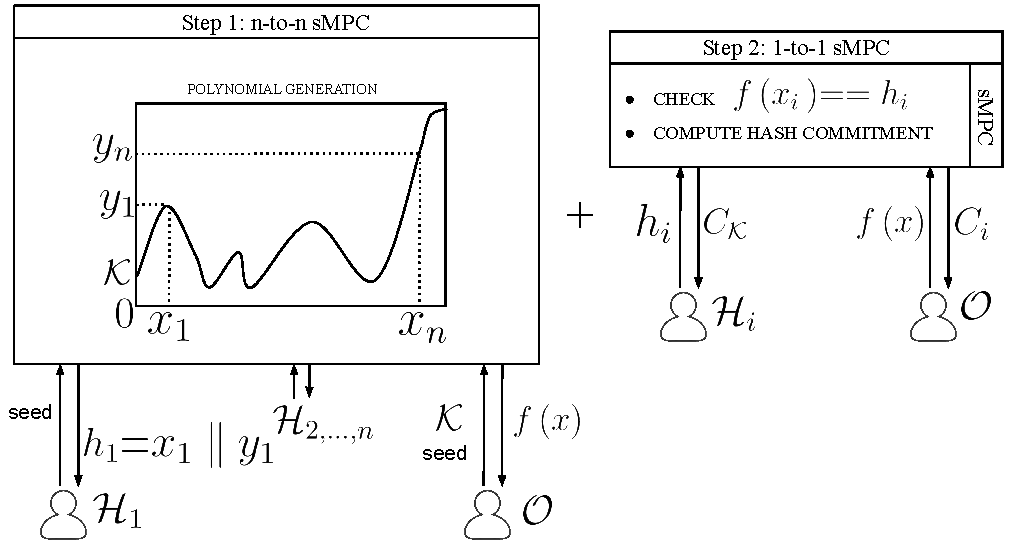
\includegraphics[width=0.8\columnwidth]{fig/mpc_rev_2}

	\caption{Two-phases sMPC protocol: step 1 jointly computed between all the parties, step 2 between owner and each shareholder.}\vspace*{-2pt}
	\label{fig:mpc2}%
\end{figure}

Our experiments are organized in two branches: simulation of \shortname instances and execution of sMPC network protocols. 
Before going into details we point out that all the results were achieved by using 256-bit shares and MiMC~\cite{albrecht2016mimc} to produce commitments. 
MiMC is a minimal multiplicative complexity hashing primitive, the advantage of its use is twofold: low gas price spent in contract calls, and lower sMPC execution time.

\medskip

\paragraph*{Simulation of \shortname instances}
A preliminary version of \shortname smart contract was derived by the use of FSolidM~\cite{Mavridou2017DesigningSE}, a framework which automatically generates Ethereum smart contracts code from a high level Finite State Machine (FSM) representation.
To deploy, test and debug the contract created, we relied on Brownie~\cite{brownie}; a framework which creates a persistent environment with which it is possible to interact through RPC. 
Brownie also permits to create wallets, inspect transactions and simulate the execution of real use cases pre-configured by Python scripts.

The experiments carried out mainly focus on the estimate of the total cost of execution of each \shortname instance. 
Figure~\ref{fig:costfigs} shows the total execution gas cost in dollars, for each role, depending on the number of \shortname participants. 
The costs were calculated by applying the exchange rate {1 ETH $=$ 221.22 USD}.
Also, Figure~\ref{fig:costfigs} reports two alternatives for the shareholder: {\em passive} and {\em active}. 
This distinction is due to the fact that many \shortname actions imply writing to the blockchain of a change of the state of the protocol.
In our simulations we have delegated all these operations to only one out of the $n$ shareholders: the active one. 
All the others have instead been classified as passive, or rather those who carry out only actions required for the success of the protocol.
By the previous differentiation it is possible to highlight an upper and a lower cost bound.
Furthermore, from the owner's perspective the total cost of execution is linear in the number of shareholders, for $n \leq 10$, while contract deployment cost is 9.18 USD.

\begin{figure*}[t]
	\centering
	\subfloat[Single-phase vs Two-phases]{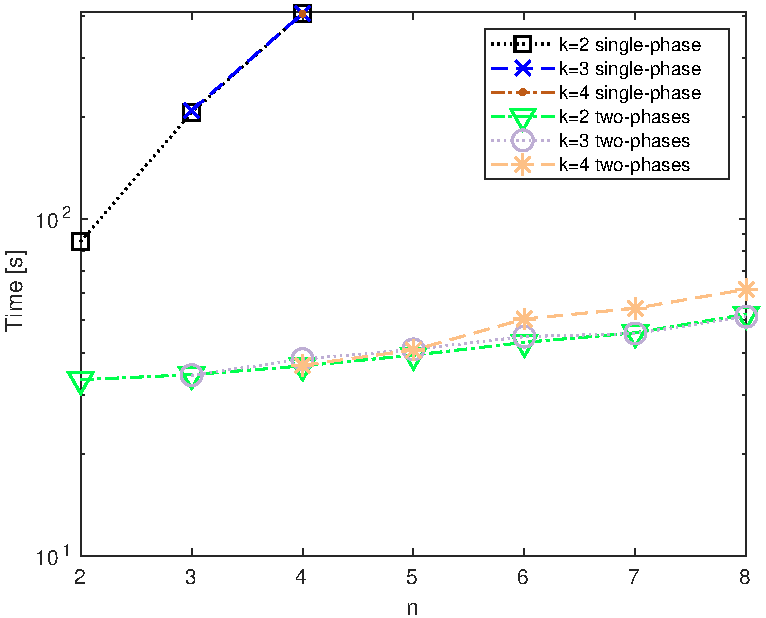
\includegraphics[width=.3\columnwidth]{fig/1a}}
	\hfill
	\subfloat[Two-phases time detail]{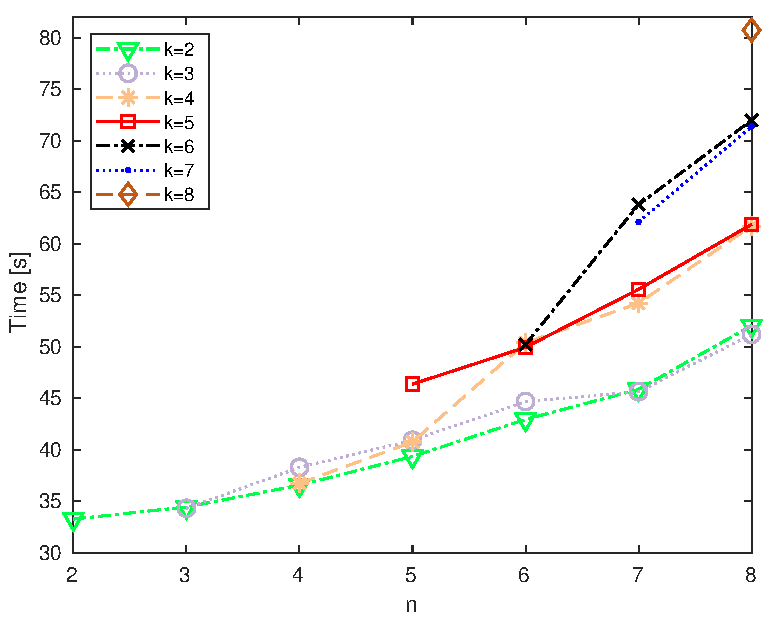
\includegraphics[width=.3\columnwidth]{fig/1b}}
	\hfill
	\subfloat[Two-phases maximum memory usage]{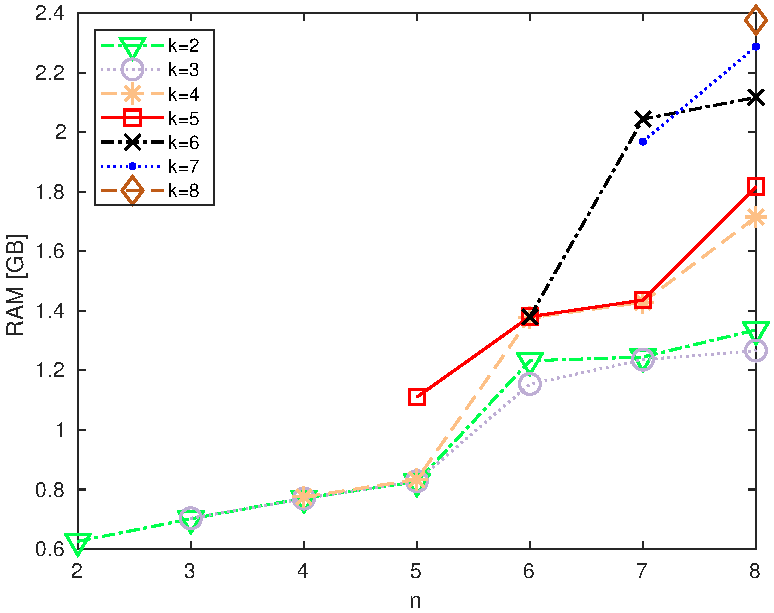
\includegraphics[width=.3\columnwidth]{fig/1c}}
	\caption{sMPC execution time and maximum memory consumption for each participant, in detail: (a) comparison between single-phase and two-phases maximum execution time, (b) two-phases execution time and (c) maximum memory consumption for higher SSS polynomial degree.}
	\label{fig:timecomp}
\end{figure*}

\medskip

\paragraph*{sMPC protocols}
The sMPC protocols were built upon FRESCO~\cite{FRESCO-git}~\cite{damgaard2016mpc}, a Framework for Efficient and Secure COmputation. Specifically, we implemented two sMPC alternatives: a {\em single-phase}, and a {\em two-phases} one. 
The single-phase one is fully compliant with the description of Section~\ref{sect:impl_mpc_brief} (briefly, \owner inputs \key and gets the commitments of all shares; while each $\shareholder_{i}$ inputs a point $x$ and receives her $\share_{i}$ plus the commitment of the key). 
On the other hand, the two-phases is made up of two subsequent sMPC protocols:
\begin{itemize}
	\item {\em Step 1} n-to-n sMPC jointly computed by all participants. The owner inputs \key and receives the polynomial function $f\left( x \right)$ generated inside the sMPC, while each shareholder inputs the point $x$ and receives her share (see Figure~\ref{fig:mpc1}). 
	\item {\em Step 2} 1-to-1 sMPC computed between the owner and each shareholder. The owner inputs $f\left( x \right)$ and receives the commitment of the $i$-th share, $\commitment_i$, while the $i$-th shareholder inputs the point $x$ plus the share $\share_{i}$, and receives the commitment of the key (see Figure~\ref{fig:mpc2}).
\end{itemize}


\begin{figure*}[t]
	\centering
	\subfloat[]{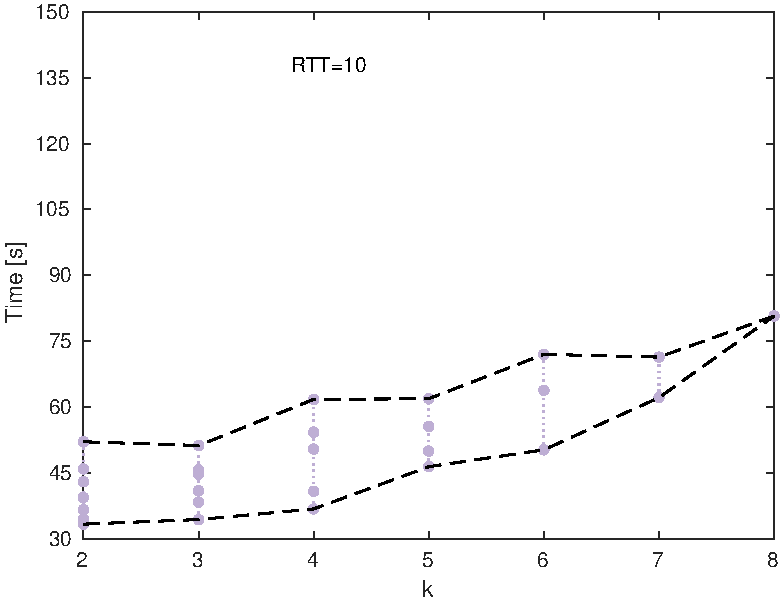
\includegraphics[width=.3\columnwidth]{fig/2a}}
	\hfill
	\subfloat[]{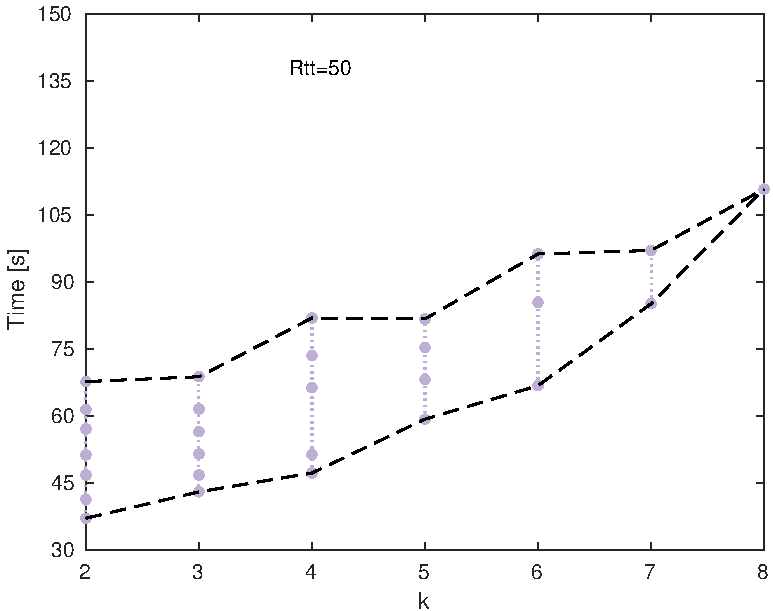
\includegraphics[width=.3\columnwidth]{fig/2b}}
	\hfill
	\subfloat[]{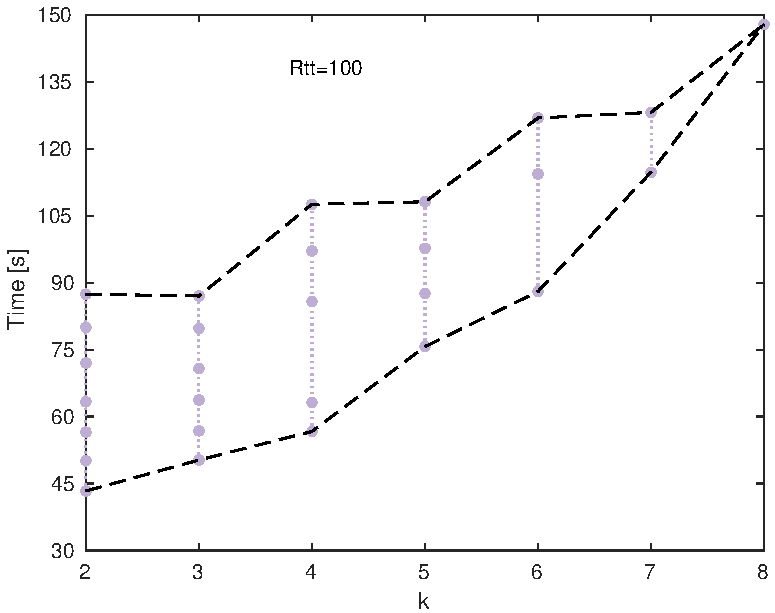
\includegraphics[width=.3\columnwidth]{fig/2c}}
	\caption{sMPC total execution time for different round trip times (Rtt) and SSS polynomial degree.}
	\label{fig:timertt}
\end{figure*}


As the reader can notice, the difference between the two sMPC alternatives lies in the calculation of the hash primitive. 
Unlike the single-phase version, the two-phases solution permits to separate Shamir polynomial generation from the production of commitments.
The benefit that follows is that, in the two-phases variant, step 1 can be implemented using boolean circuit based sMPC, while step 2 can be realized through arithmetic based sMPC.
A comparison between of total sMPC execution time of the two alternatives in shown in Figure~\ref{fig:timecomp}a, while Figure~\ref{fig:timecomp}b and Figure~\ref{fig:timecomp}c detail the maximum sMPC execution time and maximum memory consumption in case of higher SSS polynomial degree, for each participant, in two-phases solution. 

The tests have been executed on an dual Intel Xeon E5 server with 256 GB memory and SSD drive running Ubuntu 18.04 LTS.
For each \shortname participant, a different server was established, and the network communication round trip time (Rtt) was set to 10 ms (Figure~\ref{fig:timecomp}). 
To measure the effect of Rtt, we repeated the execution of all network protocols with different latency values, Figure~\ref{fig:timertt} shows a subset of the data collected for the two-phases solution (see the repository for full detail).   
However, for an exhaustive analysis on the impact of environmental parameters over sMPC implementing secret sharing cryptography we remind the reader to~\cite{DBLP:journals/corr/abs-1804-03548}.












